\section{Auswertung}
\label{sec:Auswertung}

% % Examples
% \begin{equation}
%   U(t) = a \sin(b t + c) + d
% \end{equation}
%
% \begin{align}
%   a &= \input{build/a.tex} \\
%   b &= \input{build/b.tex} \\
%   c &= \input{build/c.tex} \\
%   d &= \input{build/d.tex} .
% \end{align}
% Die Messdaten und das Ergebnis des Fits sind in Abbildung~\ref{fig:plot} geplottet.
%
% %Tabelle mit Messdaten
% \begin{table}
%   \centering
%   \caption{Messdaten.}
%   \label{tab:data}
%   \sisetup{parse-numbers=false}
%   \begin{tabular}{
% % format 1.3 bedeutet eine Stelle vorm Komma, 3 danach
%     S[table-format=1.3]
%     S[table-format=-1.2]
%     @{${}\pm{}$}
%     S[table-format=1.2]
%     @{\hspace*{3em}\hspace*{\tabcolsep}}
%     S[table-format=1.3]
%     S[table-format=-1.2]
%     @{${}\pm{}$}
%     S[table-format=1.2]
%   }
%     \toprule
%     {$t \:/\: \si{\milli\second}$} & \multicolumn{2}{c}{$U \:/\: \si{\kilo\volt}$\hspace*{3em}} &
%     {$t \:/\: \si{\milli\second}$} & \multicolumn{2}{c}{$U \:/\: \si{\kilo\volt}$} \\
%     \midrule
%     \input{build/table.tex}
%     \bottomrule
%   \end{tabular}
% \end{table}
%
% % Standard Plot
% \begin{figure}
%   \centering
%   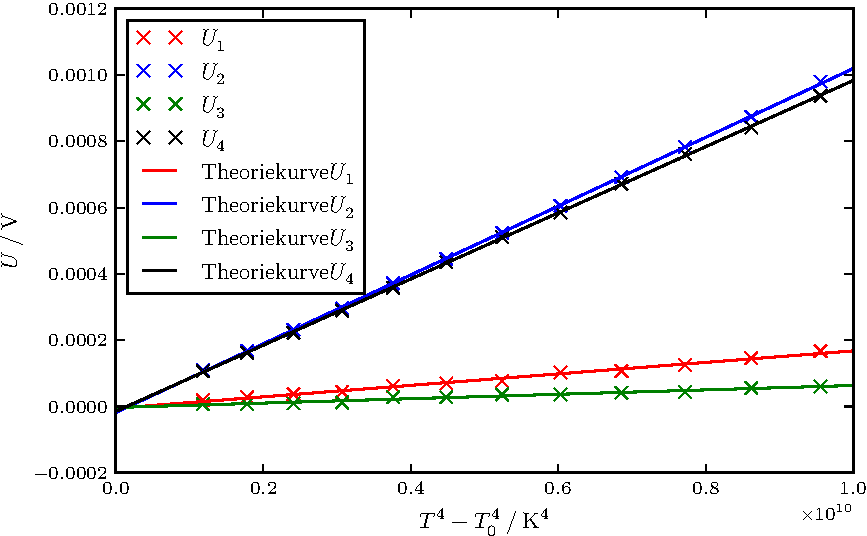
\includegraphics{build/plot.pdf}
%   \caption{Messdaten und Fitergebnis.}
%   \label{fig:plot}
% \end{figure}
%
% 2x2 Plot
% \begin{figure*}
%     \centering
%     \begin{subfigure}[b]{0.475\textwidth}
%         \centering
%         \includegraphics[width=\textwidth]{Abbildungen/Schaltung1.pdf}
%         \caption[]%
%         {{\small Schaltung 1.}}
%         \label{fig:Schaltung1}
%     \end{subfigure}
%     \hfill
%     \begin{subfigure}[b]{0.475\textwidth}
%         \centering
%         \includegraphics[width=\textwidth]{Abbildungen/Schaltung2.pdf}
%         \caption[]%
%         {{\small Schaltung 2.}}
%         \label{fig:Schaltung2}
%     \end{subfigure}
%     \vskip\baselineskip
%     \begin{subfigure}[b]{0.475\textwidth}
%         \centering
%         \includegraphics[width=\textwidth]{Abbildungen/Schaltung4.pdf}    % Zahlen vertauscht ... -.-
%         \caption[]%
%         {{\small Schaltung 3.}}
%         \label{fig:Schaltung3}
%     \end{subfigure}
%     \quad
%     \begin{subfigure}[b]{0.475\textwidth}
%         \centering
%         \includegraphics[width=\textwidth]{Abbildungen/Schaltung3.pdf}
%         \caption[]%
%         {{\small Schaltung 4.}}
%         \label{fig:Schaltung4}
%     \end{subfigure}
%     \caption[]
%     {Ersatzschaltbilder der verschiedenen Teilaufgaben.}
%     \label{fig:Schaltungen}
% \end{figure*}

\subsection{Bestimmung des Winkels der Prismaecke}
Zunächst wird, wie in der Durchführung angegeben, der dort beschriebene Winkel $\phi$ ermittelt.
Aus geometrischen Überlegungen ergibt sich dieser Winkel aus
\begin{equation}
  \varphi = \frac{1}{2} ( \varphi_l - \varphi_r)
\end{equation}
wobei $\varphi_l$ und $\varphi_r$ die in Abbildung \ref{fig:2} dargestellen Winkel sind.
Es werden die Werte
\begin{align*}
  \varphi_l &= \input{build/phi_l.tex},\\
  \varphi_r &= \input{build/phi_r.tex}
\end{align*}
gemessen, woraus sich ein Winkel von
\begin{align*}
  \varphi &= \input{build/phi.tex}
\end{align*}
ergibt.
Aufgrund der Kenntnis des realen Winkels wird im folgenden nicht mit dem gemessenen Wert, sondern mit einem Wert von $\phi = \SI{60}{\degree}$ weitergerechnet.

\subsection{Bestimmung der Brechungsindices}
Die Brechungsindices werden, wie in der Durchführung beschrieben, bestimmt.
Zunächst wird dabei die Richtungsänderung $\eta$ des Strahls berechnet, welche sich elementargeometrisch aus dem Wert
\begin{align}
  \eta = 2 (\Omega_l - \Omega_r)
\end{align}
ergibt.
Hierbei beschreiben $\Omega_l$ und $\Omega_r$ die in der Durchführung erwähnten Winkel, die sich aus den beiden symmetrischen Messungen ergeben.
Aus weiteren geometrischen Überlegungen sowie unter Verwendung von \eqref{eqn:snel} bestimmt sich der Brechungsindex $n$ zu
\begin{align}
  n = \frac{\sin{(\frac{\eta + \varphi}{2})}}{\sin{(\frac{\varphi}{2})}}.
\end{align}
Es ergeben sich für die Spektrallinien der verschiedenen Wellenlängen $\lambda$ die in Tabelle \ref{tab1} angegebenen Werte.
Die Wellenlängen werden für Quecksilber dem Versuchsaufbau sowie für Cadmium der Literatur \cite{cd} entnommen.
    \input{build/tab1_tex.tex}

\subsection{Zuordnung einer Dispersionskurve}
In der Theorie werden die beiden Möglichkeiten \eqref{eqn:d1} und \eqref{eqn:d2} als mögliche Entwicklungen einer Dispersionsrelation angegeben.
Für beide Varianten wird die Summe der Abweichungsquadrate in 2. Ordnung zu
\begin{align*}
  s_n^2 = \frac{1}{z-2} \sum ( n^2 - A_0 - \frac{A_2}{\lambda_i^2} )^2
\end{align*}
für die erste Variante bzw. zu
\begin{align*}
  s_n'^2 = \frac{1}{z-2} \sum ( n^2 - A_0' + A_2' \lambda_i^2 )^2
\end{align*}
für die zweite Variante berechnet, wobei über die $z$ Messwertpaare summiert wird.
Diese Werte geben einen Anhaltspunkt für die Übereinstimmung der Messwerte mit dem Fit.
Es ergeben sich Abweichungsquadrate von
\begin{align*}
  s_1^2 &= \input{build/Varianz_Methode_1.tex},\\
  s_2^2 &= \input{build/Varianz_Methode_2.tex}.
\end{align*}
Dementsprechend eignet sich die Dispersionsrelation mit einer positiven Krümmung besser für die vorliegenen Messdaten.\\
In 4. Ordnung werden mithilfe von SciPy in Python die Fitparameter für die Funktion \eqref{eqn:d1} bestimmt.
Es ergeben sich die Parameter
\begin{align*}
A_0 &= \input{build/A_0.tex},\\
A_2 &= \input{build/A_2.tex},\\
A_4 &= \input{build/A_4.tex},
\end{align*}
sowie eine Fitfunktion, die zusammen mit den Messdaten in Abbildung \ref{fig:4} dargestellt ist.

\begin{figure}
  \centering
  \includegraphics[height=10cm]{build/plot_a_1.pdf}
  \caption{Fit einer konkaven Dispersionskurve in 4. Ordnung.}
  \label{fig:4}
\end{figure}

\subsection{Bestimmung der Abbeschen Zahl}
Die abbesche Zahl ist definiert als
\begin{equation}
  \nu = \frac{n_D -1}{n_F - n_C},
\end{equation}
wobei $n_i$ den Brechungsindex für die Wellenlänge der jeweligen Frauenhofscher Linie bezeichnet.
Diese sind gegeben als
\begin{align*}
  \lambda_C &= \SI{656}{\nano\metre}, \\
  \lambda_D &= \SI{589}{\nano\metre}, \\
  \lambda_F &= \SI{486}{\nano\metre}.
\end{align*}
Die Brechungsindices werden der Fitfunktion entnommen, so dass sich für das hier verwendete Glasprisma ein Wert von
\begin{align*}
  \nu &= \input{build/abbesche_zahl.tex}
\end{align*}
ergibt.
Da die abbesche Zahl kleiner als 50 ist, handelt es sich beim Prisma um optisches Flintglas.
Dieses ist durch einen hohen Brechungsindex gekennzeichnet und eignet sich dementsprechend gut zur Verwendung in Prismen.

\subsection{Bestimmung des Auflösungsvermögen des Prismas}
Das Auflösungsvermögen des Primas ist definiert als
\begin{align*}
  A = \frac{\bar{\lambda}}{\increment \lambda}
\end{align*}
mit dem Wellenlängenunterschied von zwei Spektrallinien $\increment \lambda$ sowie der gemittelten Wellenlänge $\bar{\lambda}$.
Das Auflösungsvermögen ist dementsprechend ein Maß dafür, bei welcher Differenz zweier Spektrallinien eine Unterteilung dieser mit dem benutzten Prisma möglich ist.
Mithilfe der Betrachtung der Beugung an dem Prisma ist dies genau dann möglich, wenn das Hauptmaximum der Beugung der ersten Spektrallinie mindestens hinter dem ersten Minimum der zweiten Spektrallinie liegt.
Aus geometrischen Überlegungen, Berücksichtigung der Interferenzeffekte sowie geometrischen Näherungen ergibt sich das Auflösungsvermögen aus
\begin{align}
  A = b \frac{\symup{d}n}{\symup{d}\lambda}
\end{align}
mit der Basisbreite $b$ des Prismas.
Diese wird hier als $b = \SI{3}{\centi\metre}$ angenommen.
Aus der Ableitung der Fitfunktion \eqref{eqn:d2} ergeben sich für die Wellenlängen der Frauenhoferlinien $\lambda_C$ und $\lambda_F$ die Auflösungsvermögen
\begin{align*}
A_C &= \input{build/A_lambda_c.tex},\\
A_F &= \input{build/A_lambda_f.tex}.
\end{align*}

\subsection{Bestimmung einer Absorptionsstelle}
Die Absorptionsstelle ist definiert als Wellenlänge, bei der $n=0$ wird.
Unter Betrachtung von \eqref{eqn:d1} ergibt sich aus der Nullstellenbestimmung eine Absorptionsstelle bei
\begin{align*}
  \lambda_i &= \input{build/lambda_i.tex}.\\
\end{align*}
